\section{結果}
\subsubsection{揚抗力と揚抗比}
この粒子が伸びてしまうという問題(Depth-of-focus問題)を解決する策として,トモグラフィックディジタルホログラフィ法が考えられる.

\subsubsection{翼表面圧力の推定}あ
翼表面の流れ構造から翼表面圧力を推定する

\subsubsection{流れの剥離と再付着}
位相乱流強度

\subsubsection{ステレオPIVによる翼端渦構造の可視化}

\begin{figure}[H]
\centering{
\includegraphics[width=60truemm]{image/theory/tomographic.eps} %
\label{fig:tomographic}
}
\caption{Abstract of tomographic digital holography.}
\end{figure}
